\documentclass{article}

\usepackage[utf8x]{inputenc}
\usepackage{ucs}
\usepackage[portuguese]{babel}
\usepackage[T1]{fontenc}
\usepackage{amsmath}
\usepackage{amsfonts}
\usepackage{amssymb}
\usepackage{graphicx}
\usepackage{fancyhdr}
\usepackage{lastpage}
\usepackage{geometry}
\usepackage{float}
\usepackage{makecell}
\usepackage{hyperref}
\usepackage{multirow}
%\usepackage{subfigure}
\usepackage[table,xcdraw]{xcolor}
\usepackage{caption}
\usepackage{subcaption}
\usepackage{cases}
%\usepackage[framed,numbered,autolinebreaks,useliterate]{matlab-prettifier}
%\usepackage{mcode}
%\usepackage{filecontents}
\graphicspath{{Imagens/}}

% Mudando a fonte do documento para Times New Roman (ptm)
\renewcommand*\rmdefault{ptm}

\pagestyle{fancy}
\fancyhf{}
\lhead[]{Redes Neurais Artificiais}
\rhead[]{Relatório II}
\chead[]{}

\lfoot{Página \thepage \enspace de \pageref{LastPage} }
\rfoot{\leftmark}
\renewcommand{\footrulewidth}{1pt}

\usepackage{Sweave}
\begin{document}
\input{Relatorio_2-concordance}

\begin{center}

{\scshape\Large Universidade Federal de Minas Gerais \par}
{\scshape\large Redes Neurais Artificiais \par}
\vspace{5cm}

\hrule
\hfill

{\huge \textbf{ELM e RBF}\par}
\hfill
\hrule
\hfill

\vspace{3cm}

{\large\itshape Victor Marcius Magalhães Pinto\\Mat: 2019717730\par}

\vspace{2cm}

\end{center}

\newpage

\section{Introdução}

Os exercícios propostos tem por objetivo exercitar um maior conhecimento a respeito de implementações de redes neurais multicamadas, particularmente de técnicas de cálculo dos pesos. Redes ELM \textit{(Extreme Machine Learning)} baseiam-se no Teorema de Cover para realizar um remapeamento das features de entrada em um plano linearmente separável, onde a matriz de pesos de remapeamento é obtida de forma aleatória. Desta forma, ao remapear o  conjunto de dados em um um plano de maior dimensonalidade, existe uma alta probabilidade de que as classes sejam, agora, linearmente separáveis. Redes RBF, por sua vez, fazem uso de uma função de ativação radial, tipicamente oriundas de processos de clusterização, para a inicialização dos pesos da matriz de remapeamento.


\section{ELM}


\subsection{Modelagem de função de OU Exclusivo}

Usaremos ELM para modelar uma função XOR, seguindo a tabela verdade,  para u conjunto de entrada de variáveis:

% Please add the following required packages to your document preamble:
% \usepackage{graphicx}
\begin{table}[H]
\begin{tabular}{ccc}
\textbf{x1} & \textbf{x2} & \textbf{y} \\ \hline
0 & 0 & 0 \\
0 & 1 & 1 \\
1 & 0 & 1 \\
1 & 1 & 0
\end{tabular}
\end{table}

\begin{Schunk}
\begin{Sinput}
> load("data2classXOR.txt")
> rows <- dim(X)[1]
> features <- dim(X)[2]
> 
\end{Sinput}
\end{Schunk}

As features das observações podem ser entendidas como sendo valores acima ou abaixo de um determinado threshold, podendo ser modeladas como valores reais, ao invés de entradas binárias. Digamos que qualquer valor acima de 3 seja classificado como sendo 1, e abaixo como sendo 0. Desta forma a divisão das amostras pode ser vista conforme abaixo, onde a classe azul corresponde às variáveis cuja saída é 1, e a vermelha, cuja saída é 0 (ou como obtidas nos experimentos, -1).

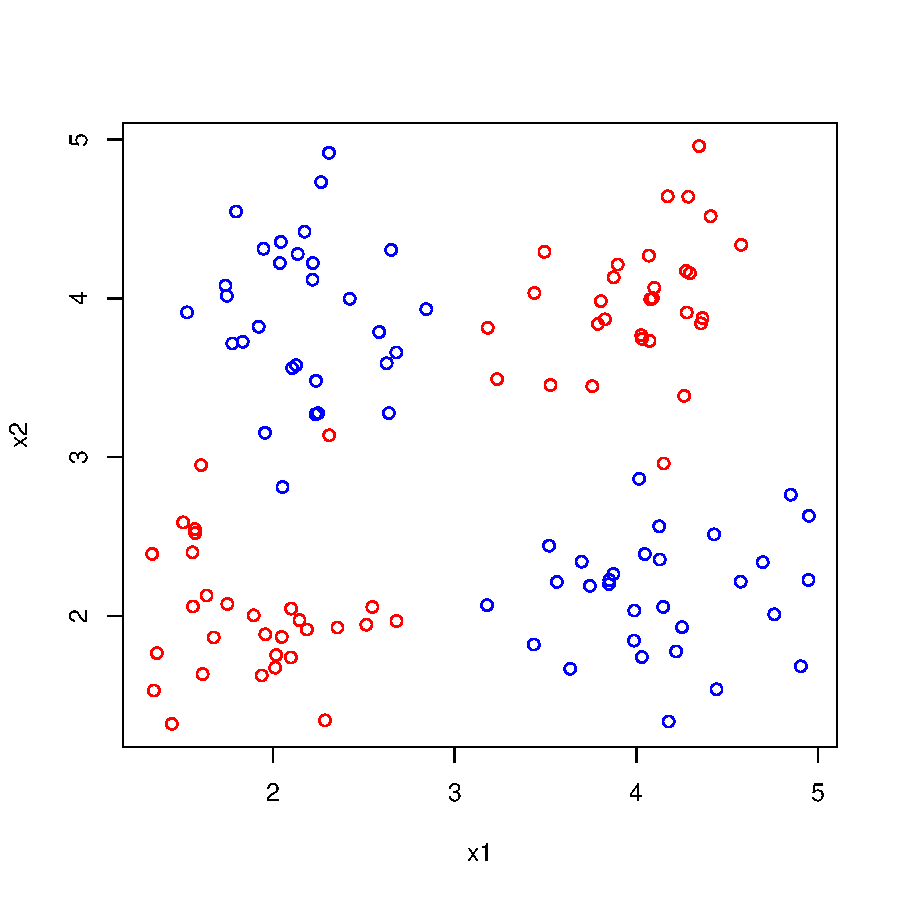
\includegraphics{Relatorio_2-003}


A rede implementada possui uma camada escondida, com 5 neurônios. O que siginifa que mapearemos cada variável, de um espaço de duas variáveis para um espaço de 5. Os pesos da matriz Z responsável pelo mapeamento das variáveis para os neurônios da camada intermediária é inicializado de forma aleatória. A partir disso, uma nova matriz de saída desta camada, remapeada, é gerada. A matriz possui dimensões iguais à quantidade de amostras de entrada pela quantidade de features novas correspondentes (número de neurônios).

\begin{Schunk}
\begin{Sinput}
> # Number of neurons in hidden layer
> p <- 5
> Z <- replicate(p, runif(features+1, -0.5, 0.5))
> print('Matriz Z')
\end{Sinput}
\begin{Soutput}
[1] "Matriz Z"
\end{Soutput}
\begin{Sinput}
> print(Z)
\end{Sinput}
\begin{Soutput}
           [,1]       [,2]       [,3]       [,4]       [,5]
[1,]  0.3491878  0.3785899 -0.3439308  0.2461366 -0.4219954
[2,]  0.4431551  0.1440150 -0.3774393 -0.2093804  0.4710252
[3,] -0.2907575 -0.2626173  0.4673047  0.2167044  0.2921702
\end{Soutput}
\begin{Sinput}
> # Adição de um termo correspondente ao bias na entrada de cada neurônio
> Xaug <- cbind(replicate(rows, 1), X)
> H <- tanh(Xaug %*% Z)
\end{Sinput}
\end{Schunk}

O cálculo da matriz de pesos, responsável por remapear as amostras, deste novo hiperplano, para os rótulos de classes corretos, é realizado através de mínimos quadrados, da saída com a pseudoinversa da saída da camada intermediária:

\begin{Schunk}
\begin{Sinput}
> W <- pseudoinverse(H) %*% Y
\end{Sinput}
\end{Schunk}

O erro para o modelo calculado é dados por:

\begin{Schunk}
\begin{Sinput}
> # Calculate Error
> Y_hat <- sign(H %*% W)
> err <- sum((Y-Y_hat)^2)/4
> print(err)
\end{Sinput}
\begin{Soutput}
[1] 12
\end{Soutput}
\end{Schunk}

Aplicando o modelo para um conjunto de teste, o erro calculado é de:

\begin{Schunk}
\begin{Sinput}
> # Test
> Xaug <- cbind(replicate(features * 4, 1), X_t)
> Ht <- tanh(Xaug %*% Z)
> Y_hat_t <- sign(Ht %*% W)
> err_t <- sum((Y_t-Y_hat_t)^2)/4
> print(err_t)
\end{Sinput}
\begin{Soutput}
[1] 6
\end{Soutput}
\end{Schunk}

A aplicação de ELM determina que mapeamos as amostras para um  espaço de dimmensionalidade muito maior do que o espaço original. Para 10 neurônios na camada escondida, temos:

\begin{Schunk}
\begin{Soutput}
[1] "Erro treinamento: 4"
\end{Soutput}
\begin{Soutput}
[1] "Erro teste: 2"
\end{Soutput}
\end{Schunk}

\noindent
para 50 neurônios,

\begin{Schunk}
\begin{Soutput}
[1] "Erro: 1"
\end{Soutput}
\begin{Soutput}
[1] "Erro teste: 4"
\end{Soutput}
\end{Schunk}


\noindent
para 100 neurônios,

\begin{Schunk}
\begin{Soutput}
[1] "Erro: 0"
\end{Soutput}
\begin{Soutput}
[1] "Erro teste: 21"
\end{Soutput}
\end{Schunk}

\noindent
para 500 neurônios,

\begin{Schunk}
\begin{Soutput}
[1] "Erro: 1"
\end{Soutput}
\begin{Soutput}
[1] "Erro teste: 3"
\end{Soutput}
\end{Schunk}

De forma geral, temos, para o treinamento, a seguinte :


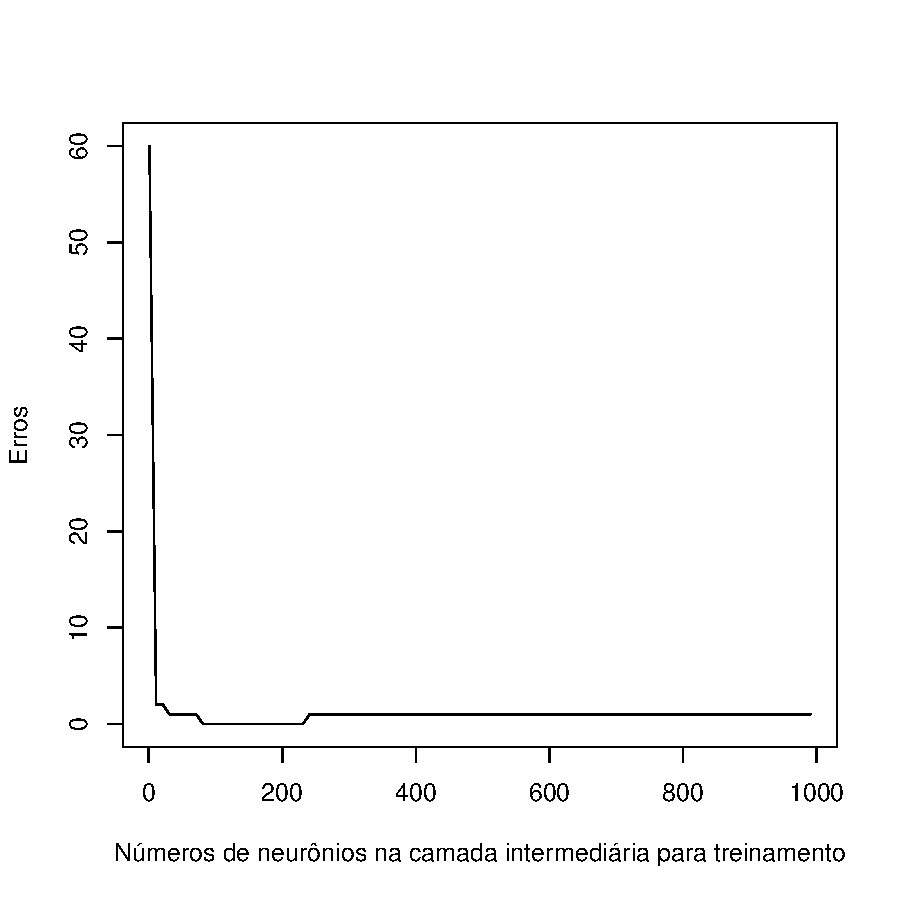
\includegraphics{Relatorio_2-012}

E, para as amostras de teste,

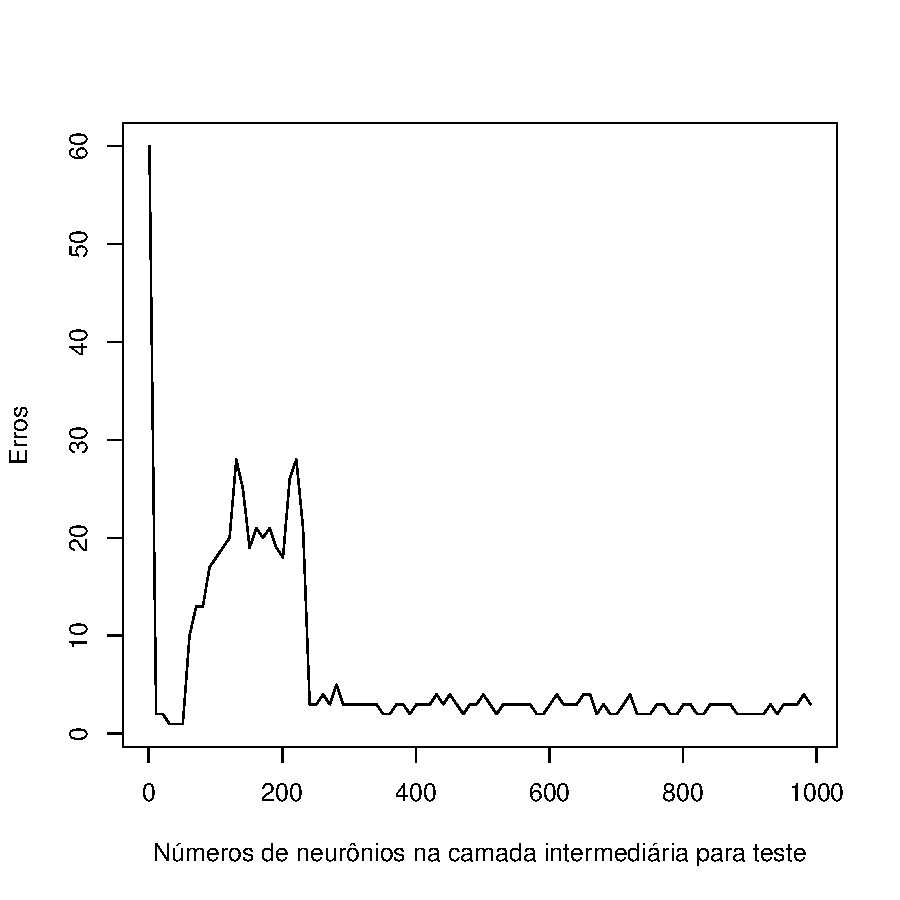
\includegraphics{Relatorio_2-013}

Os gráficos dos erros de treinamento e teste indicam que, quanto maior a quantidade de neurônios na camada intermediária, ou seja, maior a dimensionalidade do novo espaço, menor o erro de trinamento, ou seja, maior a separabilidade das classes, porém uma maior oscilação nos erros dos testes, o que pode ser um indicativo de overfitting no modelo.

\subsection{Wisconsin Breast Cancer}

O modelo de redes neurais multicamadas ELM é, agora, utilizado para treinamento de dataset Wisconsin Breast Cancer. O dataset foi dividido em treinamento e teste.

\begin{Schunk}
\begin{Sinput}
> rm(list=ls())
> data("BreastCancer")
> bc <- BreastCancer[complete.cases(BreastCancer),]
> x <- bc[, 2:10]
> y <- bc[,11]
> x <- sapply(x, as.numeric)
> y <- replicate(dim(bc)[1], 0)
> y[which(bc[,11]== 'benign')] = -1
> y[which(bc[,11]== 'malignant')] = 1
> index_train = sample(seq(dim(x)[1]), as.integer(0.7*dim(x)[1]), replace=FALSE)
> x_train = x[index_train,]
> x_test = x[-index_train,]
> y_train <- y[index_train]
> y_test = y[-index_train]
\end{Sinput}
\end{Schunk}

Para avaliar o resultado das operações, será feito uso de uma função de performance, especificada como abaixo:

\begin{Schunk}
\begin{Sinput}
> evaluate <- function(y, y_hat) {
+ 
+     y[which(y<0)] = 0
+     y_hat[which(y_hat<0)] = 0
+ 
+     errors <- y - y_hat
+     false_positive <- length(errors[errors < 0])
+     true_positive <- length(y[y[which(errors == 0)] > 0])
+     false_negative <- length(errors[errors > 0])
+     true_negative <- length(y[y[which(errors == 0)] <= 0])
+ 
+     confusion_matrix <- matrix(replicate(4, 0), nrow = 2, ncol = 2)
+     confusion_matrix[1,1] <- true_positive
+     confusion_matrix[1,2] <- false_positive
+     confusion_matrix[2,1] <- false_negative
+     confusion_matrix[2,2] <- true_negative
+ 
+     return(list(
+         'errors' = errors,
+         'error'= mean(abs(errors)),
+         'accuracy' = (1 - mean(abs(errors))),
+         'specitivity'= true_negative / (true_negative + false_positive),
+         'sensibility' = true_positive / (true_positive + false_negative),
+         'confusion_matrix' = confusion_matrix
+     ))
+ }
\end{Sinput}
\end{Schunk}


Realizando o treinamento, temos as seguintes métricas como resultado.

\begin{Schunk}
\begin{Soutput}
[1] "Porcentagem de erro: 0.098326"
\end{Soutput}
\begin{Soutput}
[1] "Acurácia: 0.901674"
\end{Soutput}
\begin{Soutput}
[1] "Sensibiliade: 0.835294"
\end{Soutput}
\begin{Soutput}
[1] "Especificidade: 0.946479"
\end{Soutput}
\end{Schunk}

As métricas de teste obtidas mostram um bom desempenho do modelo para a predição de câncer de mama, com as features especificadas. A matriz de confusão obtida pode ser vista a seguir:

\begin{Schunk}
\begin{Soutput}
     [,1] [,2]
[1,]  142   19
[2,]   28  336
\end{Soutput}
\end{Schunk}

A matriz de confusão corresponde a:

\begin{table}[H]
\begin{tabular}{|l|l|}
\hline
True Positive & False Positive \\ \hline
False Negative & True Negative \\ \hline
\end{tabular}
\end{table}

\section{RBF}

Redes RBF, como mencionado anteriormente, utilizam funções de ativação radial para os neurônios da camada escondida. A saída da rede, constituindo-se de um valor único, é definida como sendo:

\begin{equation}
\varphi(\overline{X}) = \sum^{N}_{i=1} \alpha_i \rho(|| \overline(x) - \overline(c)_i ||)
\end{equation}





\begin{thebibliography}{1}

	%Each item starts with a \bibitem{reference} command and the details thereafter.
	\bibitem{specificity} % Transaction paper
	ML Metrics: Sensitivity vs. Specificity -
	\url{https://dzone.com/articles/ml-metrics-sensitivity-vs-specificity-difference}.
	Acessado em 28 de agosto de 2019.


\end{thebibliography}

\end{document}
